% VUT FIT MITAI
% MSZ 2021/2022
% Author: Vladimir Dusek
% Login: xdusek27

%%%%%%%%%%%%%%%%%%%%%%%%%%%%%%%%%%%%%%%%%%%%%%%%%%%%%%%%%%%%%%%%%%%%%%%%%%%%%%%%

% Path to figures
\graphicspath{{msp/regresni_analyza/figures}}

%%%%%%%%%%%%%%%%%%%%%%%%%%%%%%%%%%%%%%%%%%%%%%%%%%%%%%%%%%%%%%%%%%%%%%%%%%%%%%%%

\chapter{MSP~--~Regresní analýza.}

%%%%%%%%%%%%%%%%%%%%%%%%%%%%%%%%%%%%%%%%%%%%%%%%%%%%%%%%%%%%%%%%%%%%%%%%%%%%%%%%

\section{Zdroje}

\begin{compactitem}
    \item \path{MSP_pred_02_Opakovani_Statistika_Regrese.pdf}
    \item \path{MSP_pred_06_Regresni-analyza_Uvod.pdf}
    \item \path{MSP_pred_07_Reg-analyza_Testy_Spec-modely_Diagnostika.pdf}
    \item Wikipedia
\end{compactitem}

%%%%%%%%%%%%%%%%%%%%%%%%%%%%%%%%%%%%%%%%%%%%%%%%%%%%%%%%%%%%%%%%%%%%%%%%%%%%%%%%

\section{Úvod a kontext}

\begin{compactitem}
    \item Základní úlohou regresní analýzy je nalezení vhodného modelu studované závislosti.

    \item \textbf{Korelační analýza} se zabývá vzájemnými (většinou lineárními) závislostmi, kdy se klade důraz především na intenzitu (sílu) vzájemného vztahu než na zkoumání veličin ve směru příčina -- následek.

    \item \textbf{Regresní analýza} se zabývá jednostrannými závislostmi. Jedná se o situaci, kdy proti sobě stojí vysvětlující (nezávislá) proměnná v úloze příčin a vysvětlovaná (závislá) proměnná v úloze následků (hledání závislostí mezi atributy). V podstatě jde o aproximaci souboru dat vhodnou funkcí (tzv. regresní funkce). \begin{compactitem}
        \item Na začátku regresní analýzy je třeba odhadnout typ funkce. K tomu slouží explorativní analýza, která se používá ke zjištění, jak cílový atribut závisí na ostatních atributech (na kterých a jak).
        \item Poté je třeba určit parametry regresní funkce, například pomocí metody nejmenších čtverců.
        \item V závěru je třeba model verifikovat, zda funguje i na datech, na kterých nebyl přímo trénován.
    \end{compactitem}

    \item Rozlišujeme různé typy: \begin{compactitem}
        \item Jednoduchá lineární regrese -- Cílový atribut závisí na jednom dalším atributu lineárně.
        \item Vícenásobná lineární regrese -- Cílový atribut závisí na několika dalších atributech lineárně.
        \item Nelineární regrese -- Cílový atribut závisí na dalších atributech nelineárně.
    \end{compactitem}

\end{compactitem}

%%%%%%%%%%%%%%%%%%%%%%%%%%%%%%%%%%%%%%%%%%%%%%%%%%%%%%%%%%%%%%%%%%%%%%%%%%%%%%%%

\section{Polynomiální regrese}

\begin{compactitem}
    \item Polynomiální regrese představuje proložení (aproximaci) zadaných hodnot polynomem.

    \item Postup: \begin{compactitem}
        \item Mějme datový soubor $Y$ reprezentovaný uspořádanou n-ticí: $$Y = (y_1, y_2, \ldots, y_n)$$
        \item cílem je najít takový polynom k-tého stupně:
        $$P_k(x) = p_0 + p_1 x + \ldots + p_k x^k$$
        \item pro který platí
        $$y_i = P_k(x_i) + e_i$$
        pro $i \in 1 \ldots n$, kde $e_i$ je odchylka (nebo také chyba). Koeficienty $p_0, p_1, \ldots, p_k$ jsou přitom voleny tak, aby součet druhých mocnin odchylek, resp. suma $$\sum_{i=1}^n e_i^2$$, byla co nejmenší.
    \end{compactitem}
\end{compactitem}

\subsection{Metoda nejmenších čtverců}

\begin{figure}[H]
    \centering
    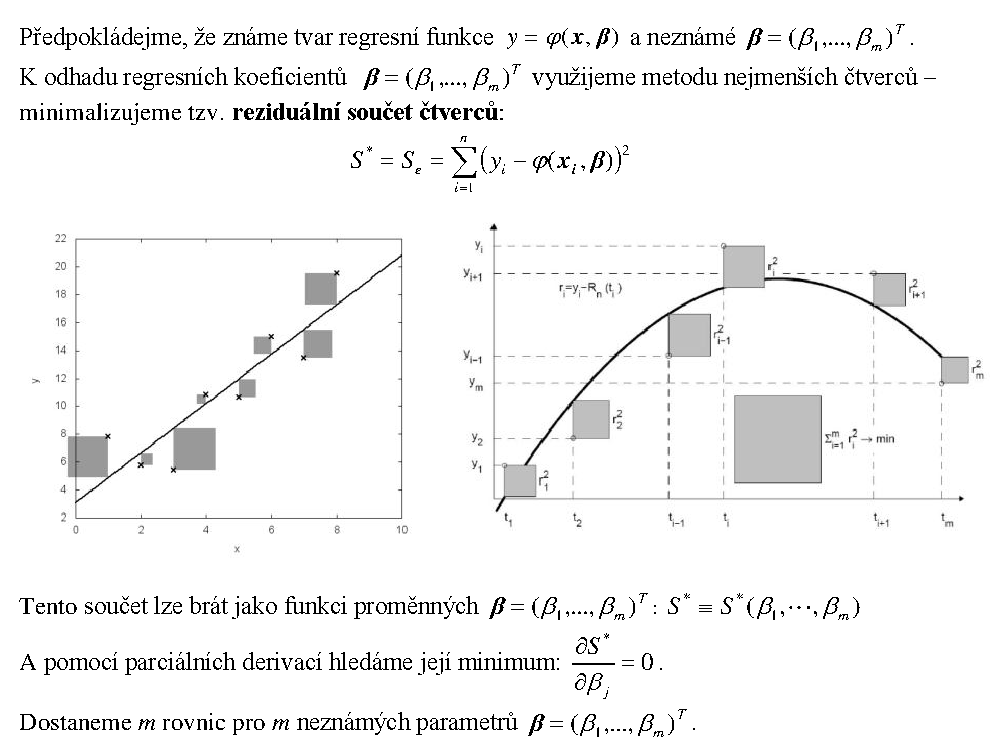
\includegraphics[width=1\linewidth]{nejmensi_ctverce.pdf}
    \caption{Odhad parametrů regresní funkce pomocí metody nejmenších čtverců.}
\end{figure}

\subsection{Střední kvadratická chyba}

\begin{compactitem}
    \item Jedna z chybových metrik je tzv. střední kvadratická chyba (MSE, \textit{Mean Squared Error}).

    \item Mějme trénovací datový soubor $(X, Y)$, kde $X = (x_1, x_2, \ldots, x_n)$ jsou hodnoty ovlivňující proměnné a $Y = (y_1, y_2, \ldots, y_n)$ jsou hodnoty cílové proměnné, a regresní funkci $f$, která aproximuje datovou sadu $(X, Y)$.

    \item Výpočet chyby MSE regresní funkce $f$ na datovém souboru $(X, Y)$:
    $$ \text{MSE} = \frac{1}{n} \sum_{i=1}^n (y_i - f(x_i))^2 $$
\end{compactitem}

%%%%%%%%%%%%%%%%%%%%%%%%%%%%%%%%%%%%%%%%%%%%%%%%%%%%%%%%%%%%%%%%%%%%%%%%%%%%%%%%

\section{Příklad: Vypočtěte bodový odhad koeficientu korelace.}

\begin{compactitem}
    \item Měřením dvojice (Výška[cm], Váha[kg]) u vybraných studentů z FIT byl získán dvourozměrný statistický soubor zapsaný po dvojicích v řádcích. Statistický soubor bude využit pro tento a všechny další příklady.
\end{compactitem}

\begin{figure}[H]
    \centering
    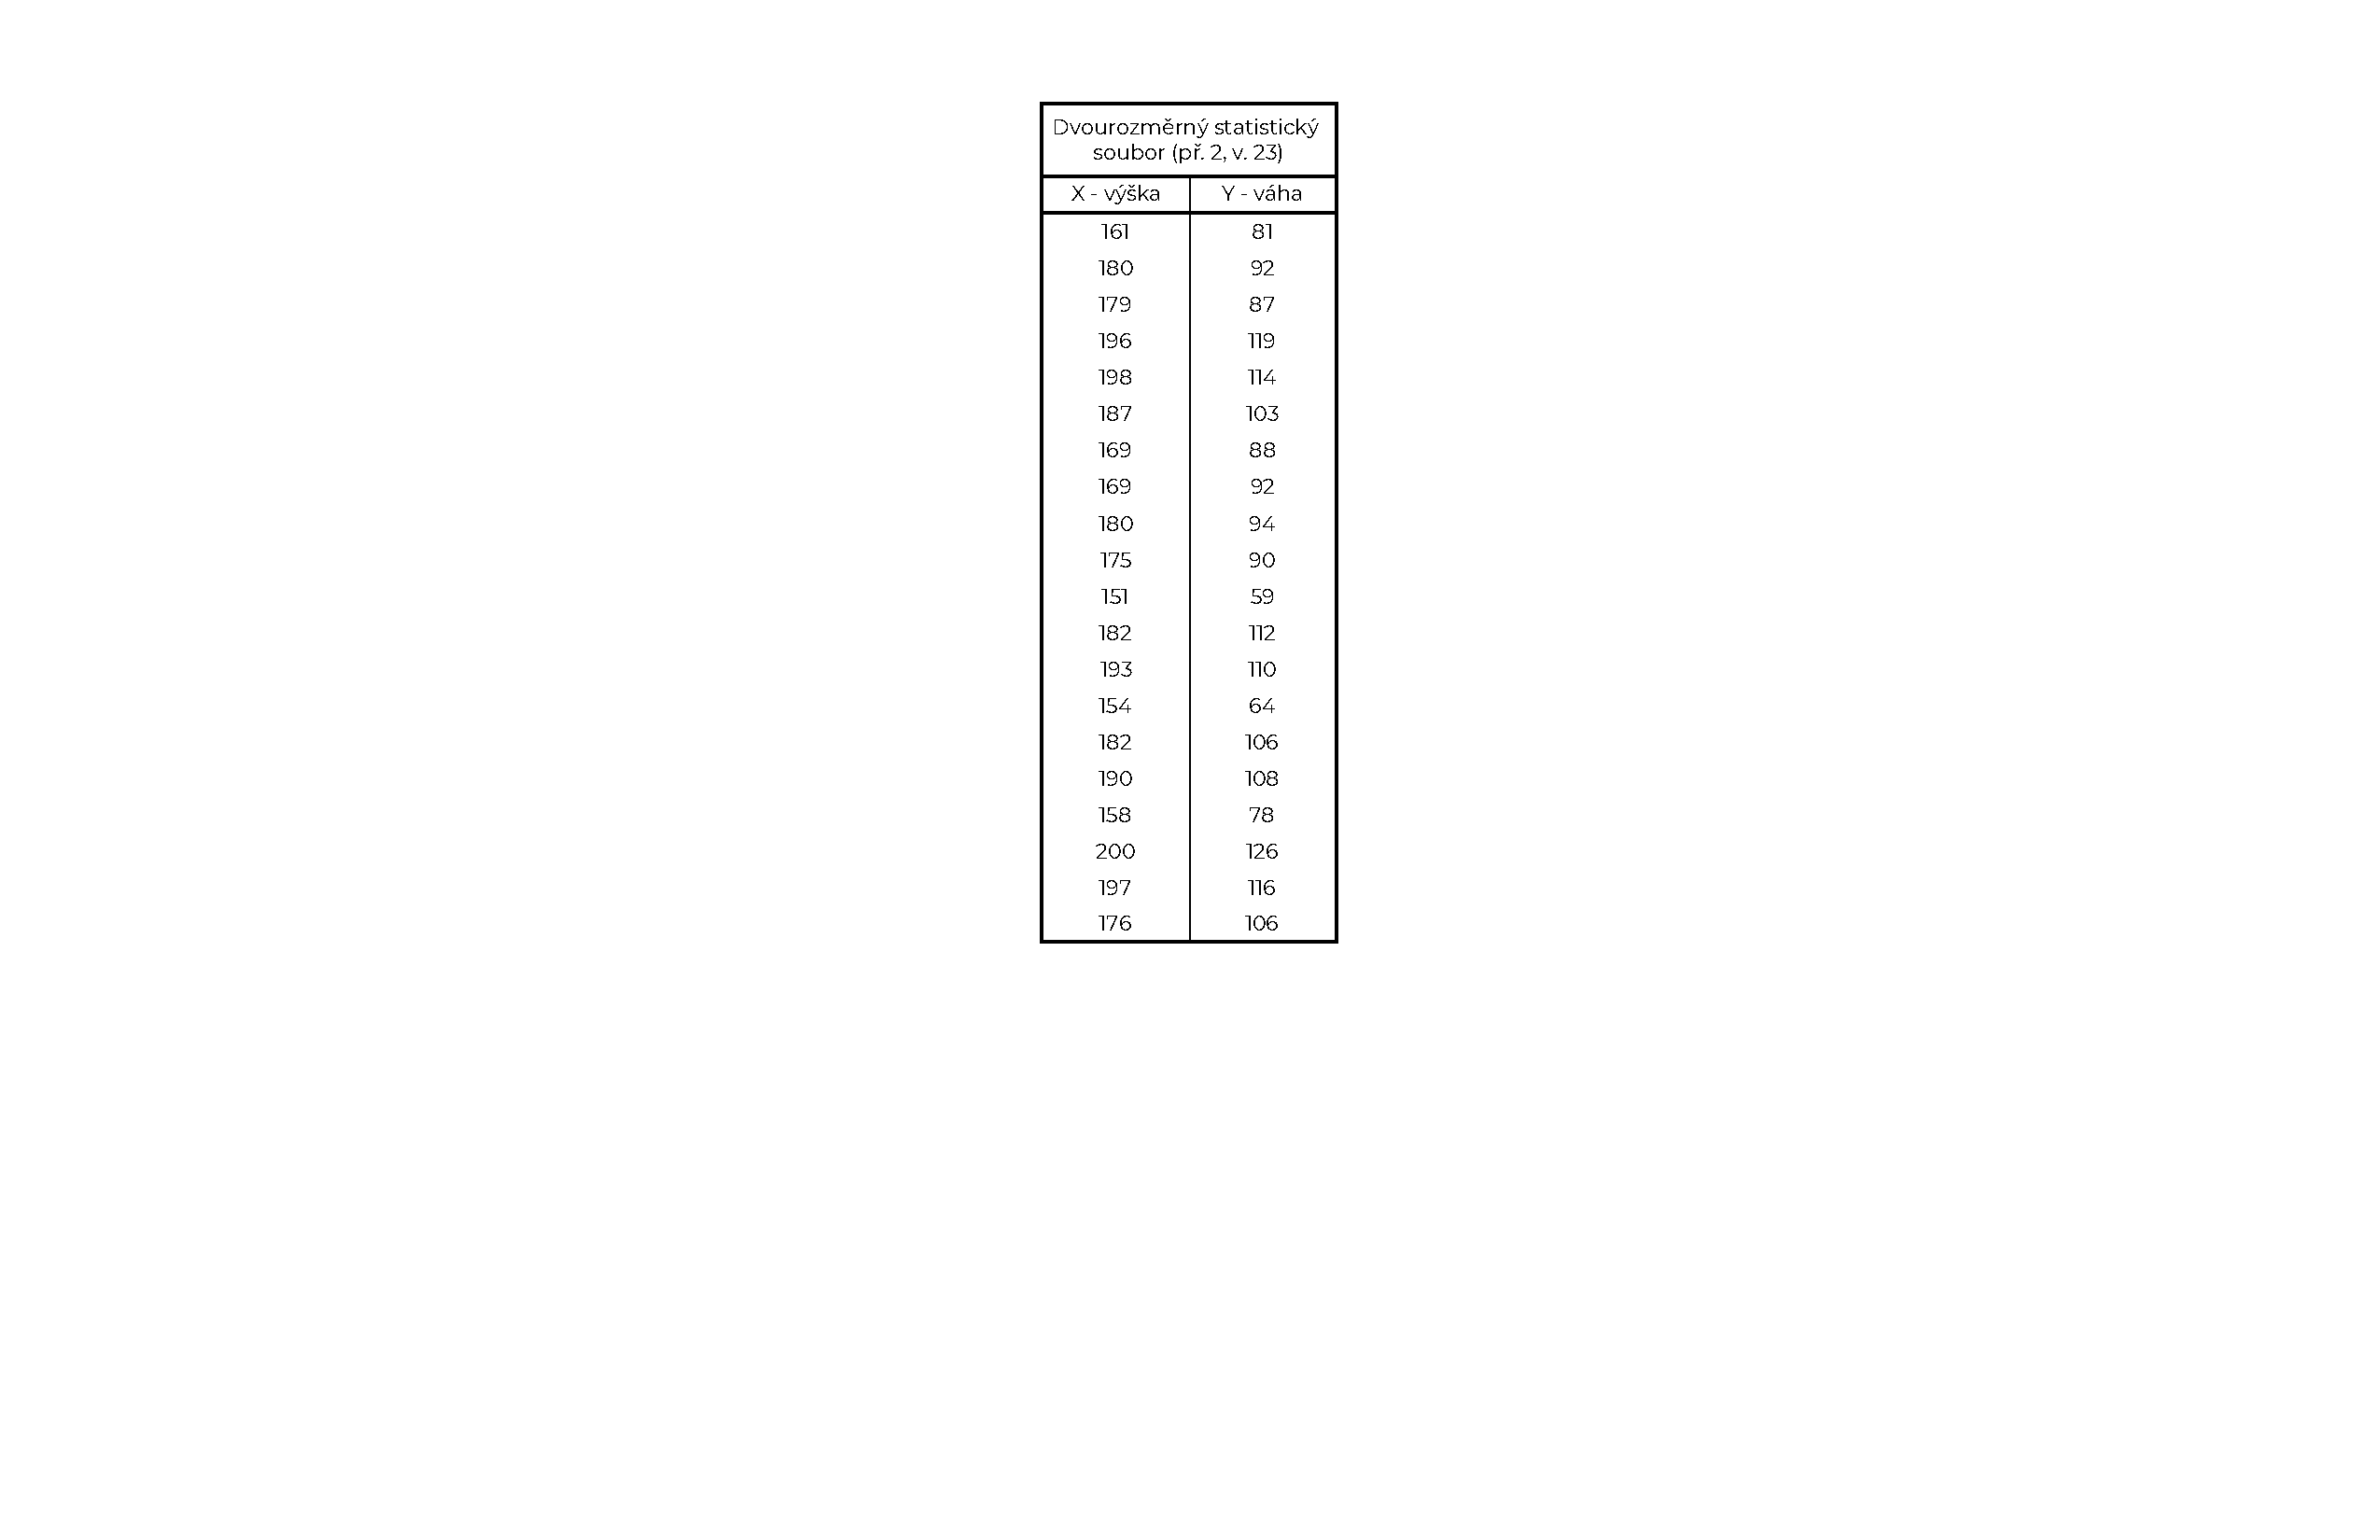
\includegraphics[width=.25\linewidth]{2-1-crop.pdf}
    \caption{Statistický soubor pro tento a všechny další příklady.}
\end{figure}

\begin{minipage}{0.49\textwidth}
    $${\displaystyle n = 20}$$
    $${\displaystyle \overline{x} = 178.85}$$
    $${\displaystyle \overline{y} = 97.25}$$
\end{minipage}
%
\begin{minipage}{0.49\textwidth}
    $${\displaystyle \sum_{i=1}^n x_i^2 = 643 \, 961}$$
    $${\displaystyle \sum_{i=1}^n y_i^2 = 195 \, 277}$$
    $${\displaystyle \sum_{i=1}^n x_i \cdot y_i = 352 \, 644}$$
\end{minipage}
\bigskip

\begin{compactitem}
    \item Odhad koeficientu korelace:
    $${\displaystyle r = \frac{\sum\limits_{i=1}^n x_i \cdot y_i - n \cdot \overline{x} \cdot \overline{y}} {\sqrt{ \bigg( \sum\limits_{i=1}^n x_i^2 - n \cdot \overline{x}^2\bigg) \cdot \bigg( \sum\limits_{i=1}^n y_i^2 - n \cdot \overline{y}^2 \bigg)}} \approx 0.9409}$$
\end{compactitem}

%%%%%%%%%%%%%%%%%%%%%%%%%%%%%%%%%%%%%%%%%%%%%%%%%%%%%%%%%%%%%%%%%%%%%%%%%%%%%%%%

\section{Příklad: Na hladině významnosti $0.05$ testujte hypotézu, že náhodné veličiny Výška a Váha jsou lineárně nezávislé.}

\begin{compactitem}
    \item Hypotéza
    $${\displaystyle H_0 : \rho = 0}$$

    \item Alternativní hypotéza
    $${\displaystyle H_A : \rho \neq 0}$$

    \item Testovací kritérium
    $${\displaystyle t = \frac{|r| \cdot \sqrt{n - 2}}{\sqrt{1 - r^2}} \approx 11.7859}$$

    \item Stupeň volnosti
    $${\displaystyle k = n - 2}$$

    \item Kvantil Studentova rozdělení pro hladinu významnosti
    ${\displaystyle \alpha = 0.05}$:

    $${\displaystyle \qquad t_{1 - \frac{\alpha}{2}}(k) = t_{0.975}(18) \approx 2.101}$$

    \item Doplněk kritického oboru pro alternativní hypotézu ${\displaystyle H_{A}}$:
    $${\displaystyle \qquad \overline{W_\alpha} = \big\langle 0 \;,\; t_{1 - \frac{\alpha}{2}}(k) \big\rangle \approx \big\langle 0 \;,\; 2.101 \big\rangle}$$

    \item Jelikož ${\displaystyle t \notin \overline{W_\alpha}}$, tak hypotéza ${\displaystyle H_0}$ se \textbf{zamítá}.
\end{compactitem}

%%%%%%%%%%%%%%%%%%%%%%%%%%%%%%%%%%%%%%%%%%%%%%%%%%%%%%%%%%%%%%%%%%%%%%%%%%%%%%%%

\section{Příklad: Regresní analýza, data proložte přímkou}

\begin{compactitem}
    \item Tvar přímky
    $${\displaystyle Vaha = \beta_0 + \beta_1 \cdot Vyska}$$

    \item Pomocné výpočty
\end{compactitem}

\begin{minipage}{0.49\textwidth}
    $${\displaystyle n = 20}$$
    $${\displaystyle \sum_{i=1}^n x_i = 3 \, 577}$$
    $${\displaystyle \sum_{i=1}^n y_i = 1 \, 945}$$
\end{minipage}
%
\begin{minipage}{0.49\textwidth}
    $${\displaystyle \sum_{i=1}^n x_i^2 = 643 \, 961}$$
    $${\displaystyle \sum_{i=1}^n y_i^2 = 195 \, 277}$$
    $${\displaystyle \sum_{i=1}^n x_i \cdot y_i = 352 \, 644}$$
\end{minipage}

$${\displaystyle
    H = \begin{pmatrix}
        n                       & \sum\limits_{i=1}^n x_i   \\
        \sum\limits_{i=1}^n x_i & \sum\limits_{i=1}^n x_i^2
    \end{pmatrix}
}$$

$${\displaystyle det(H) = n \cdot \sum_{i=1}^n x_i^2 - \Bigg( \sum_{i=1}^n x_i \Bigg)^2 = 84 \, 291}$$

\subsection{Bodový odhad koeficientů ${\displaystyle \beta_0}$, ${\displaystyle \beta_1}$ a rozptylu ${\displaystyle s^2}$}

\begin{compactitem}
    \item Hledáme lineární funkci ${\displaystyle y = \beta_0 + \beta_1 \cdot x}$, která bude nejlépe aproximovat naše naměřená data. Bodové odhady koeficientů ${\displaystyle \beta_0}$ a ${\displaystyle \beta_1}$ budeme značit ${\displaystyle b_0}$ a ${\displaystyle b_1}$.

    \item Bodový odhad koeficientů pomocí metody nejmenších čtverců
    $${\displaystyle \qquad b_1 = \frac{1} {det(H)} \cdot \Bigg( n \cdot \sum_{i=1}^n x_i \cdot y_i - \sum_{i=1}^n x_i \cdot \sum_{i=1}^n y_i \Bigg) \approx 1.1343 }$$
    $${\displaystyle \qquad b_0 = \overline{y} - b_1 \cdot \overline{x} \approx -105.6274}$$ \begin{compactitem}
        \item Regresní funkce: $${\displaystyle y = 1.1343 \cdot x - 105.6274}$$
    \end{compactitem}

    \item Bodový odhad rozptylu pomocí metody nejmenších čtverců \begin{compactitem}
        \item Minimální hodnota reziduálního součtu čtverců
        $${\displaystyle S^*_{min} = \sum_{i=1}^n y_i^2 - b_0 \cdot \sum_{i=1}^n y_i - b_1 \cdot \sum_{i=1}^n x_i \cdot y_i \approx 702.7344}$$

        \item Rozptyl
        $${\displaystyle s^2 = \frac{S^*_{min}} {n-2} \approx 39.0408}$$

    \end{compactitem}
\end{compactitem}

\subsection{Testování hypotézy ${\displaystyle H_1 : \beta_0 = -100}$}

\begin{compactitem}
    \item Alternativní hypotéza $${\displaystyle H_{1A} : \beta_0 \neq -100}$$

    $${\displaystyle h_{11} = \frac{\sum\limits_{i=1}^n x_i^2} {det(H)} \approx 7.6397}$$

    \item Testovací kritérium
    $${\displaystyle t_1 = \frac{b_0 - \beta_0}{s \cdot \sqrt{h_{11}}} \approx -0.3258}$$

    \item Stupeň volnosti
    $${\displaystyle k = n - 2}$$

    \item Kvantil Studentova rozdělení pro hladinu významnosti ${\displaystyle \alpha = 0.05}$:
    $${\displaystyle \qquad t_{1 - \frac{\alpha}{2}}(k) = t_{0.975}(18) \approx 2.101}$$

    \item Doplněk kritického oboru pro alternativní hypotézu ${\displaystyle H_{1A}}$:
    $${\displaystyle \qquad \overline{W_\alpha} = \big\langle -t_{1 - \frac{\alpha}{2}}(k) \;,\; t_{1 - \frac{\alpha}{2}}(k) \big\rangle \approx \big\langle -2.101 \;,\; 2.101 \big\rangle}$$

    \item Jelikož ${\displaystyle t_1 \in \overline{W_\alpha}}$, tak hypotéza ${\displaystyle H_1}$ se \textbf{nezamítá}.
\end{compactitem}

\subsection{Testování hypotézy ${\displaystyle H_2 : \beta_1 = 1}$}

\begin{compactitem}
    \item Alternativní hypotéza
    $${\displaystyle H_{2A} : \beta_1 \neq 1}$$

    $${\displaystyle h_{22} = \frac{n} {det(H)} \approx -0.9207}$$

    \item Testovací kritérium
    $${\displaystyle t_2 = \frac{b_1 - \beta_1}{s \cdot \sqrt{h_{22}}} \approx -0.0234}$$

    \item Doplněk kritického oboru je stejný jako u testování hypotézy ${\displaystyle H_1}$.

    \item Jelikož ${\displaystyle t_2 \in \overline{W_\alpha}}$, tak hypotéza ${\displaystyle H_2}$ se \textbf{nezamítá}.

\end{compactitem}

\subsection{Graf bodů s regresní přímkou a pásem spolehlivosti pro individuální hodnotu výšky}

\begin{compactitem}
    \item Intervalový odhad střední hodnoty $y$
    $${\displaystyle \Big\langle (b_0 + b_1 \cdot x) - t_{1 - \frac{\alpha}{2}}(k) \cdot s \cdot \sqrt{h^*} \;,\; (b_0 + b_1 \cdot x) + t_{1 - \frac{\alpha}{2}}(k) \cdot s \cdot \sqrt{h^*} \Big\rangle}$$

    \item Intervalový odhad individuální hodnoty $y$
    $${\displaystyle \Big\langle (b_0 + b_1 \cdot x) - t_{1 - \frac{\alpha}{2}}(k) \cdot s \cdot \sqrt{h^* + 1} \;,\; (b_0 + b_1 \cdot x) + t_{1 - \frac{\alpha}{2}}(k) \cdot s \cdot \sqrt{h^* + 1} \Big\rangle}$$
    kde
    $${\displaystyle h^* = \frac{1}{n} + \frac{n \cdot (x - \overline{x})^2}{det(H)}}$$
\end{compactitem}

\begin{figure}[H]
    \centering
    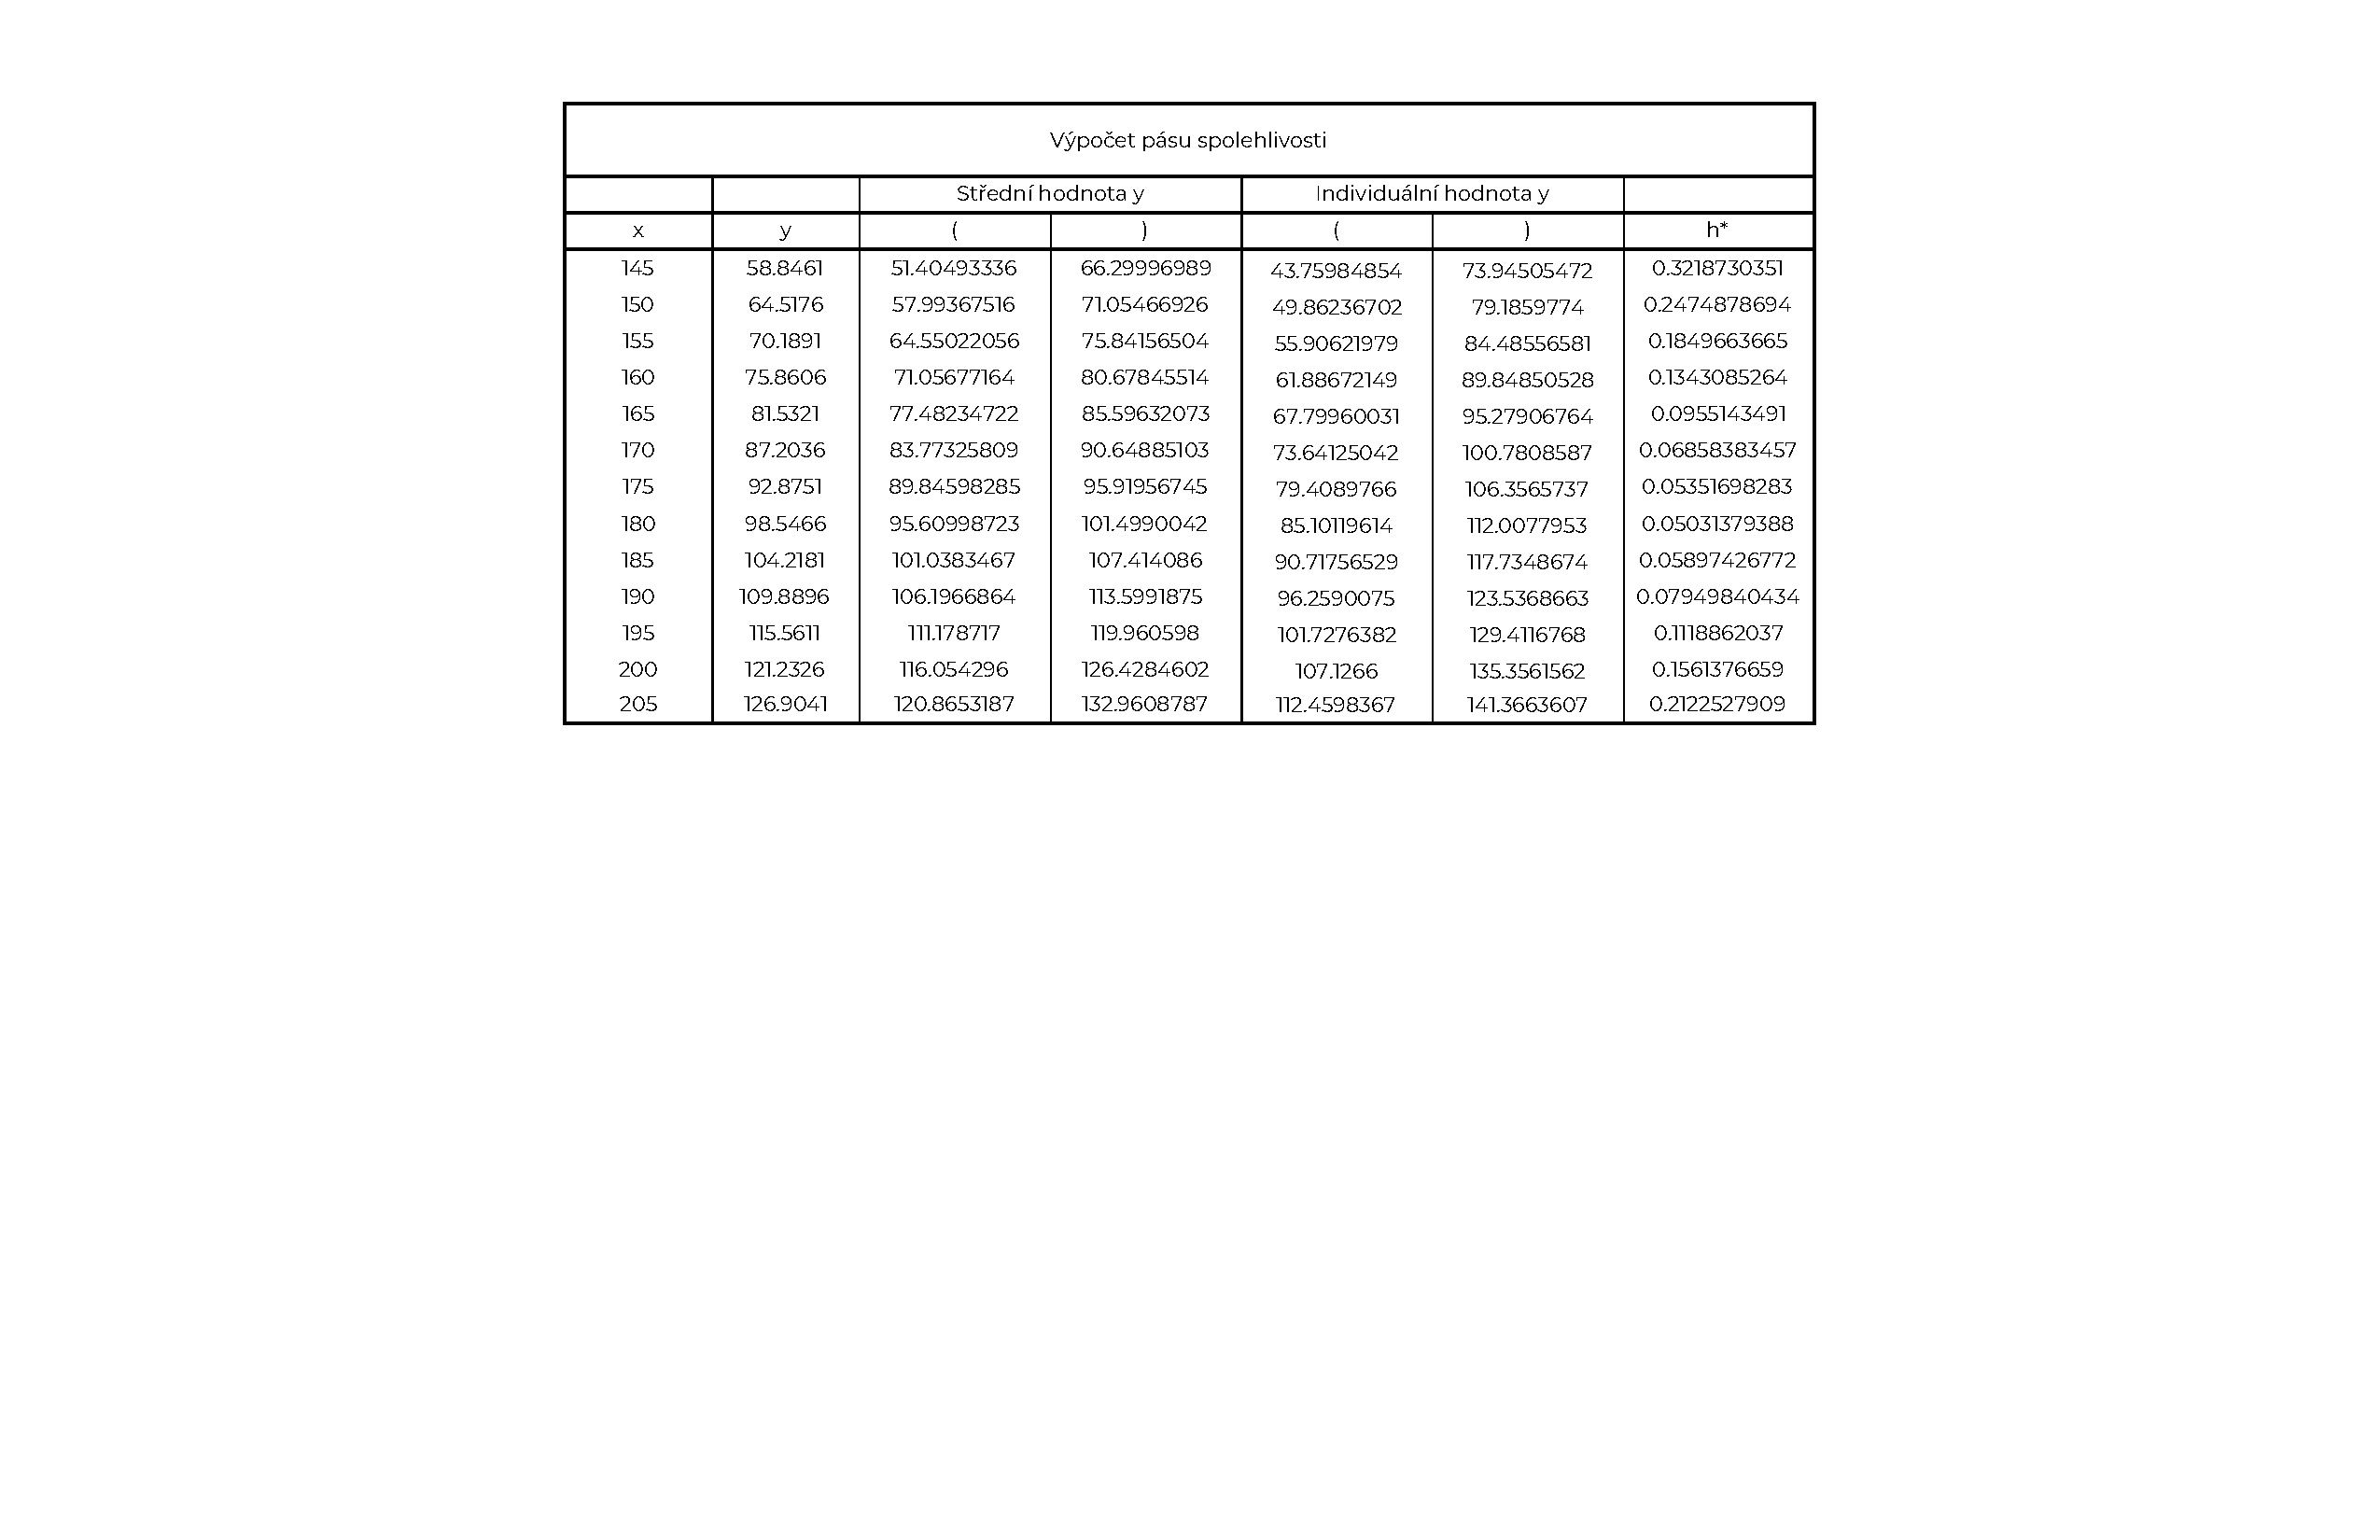
\includegraphics[width=1\linewidth]{2-c-1-crop.pdf}
\end{figure}
\bigskip

\begin{figure}[H]
    \centering
    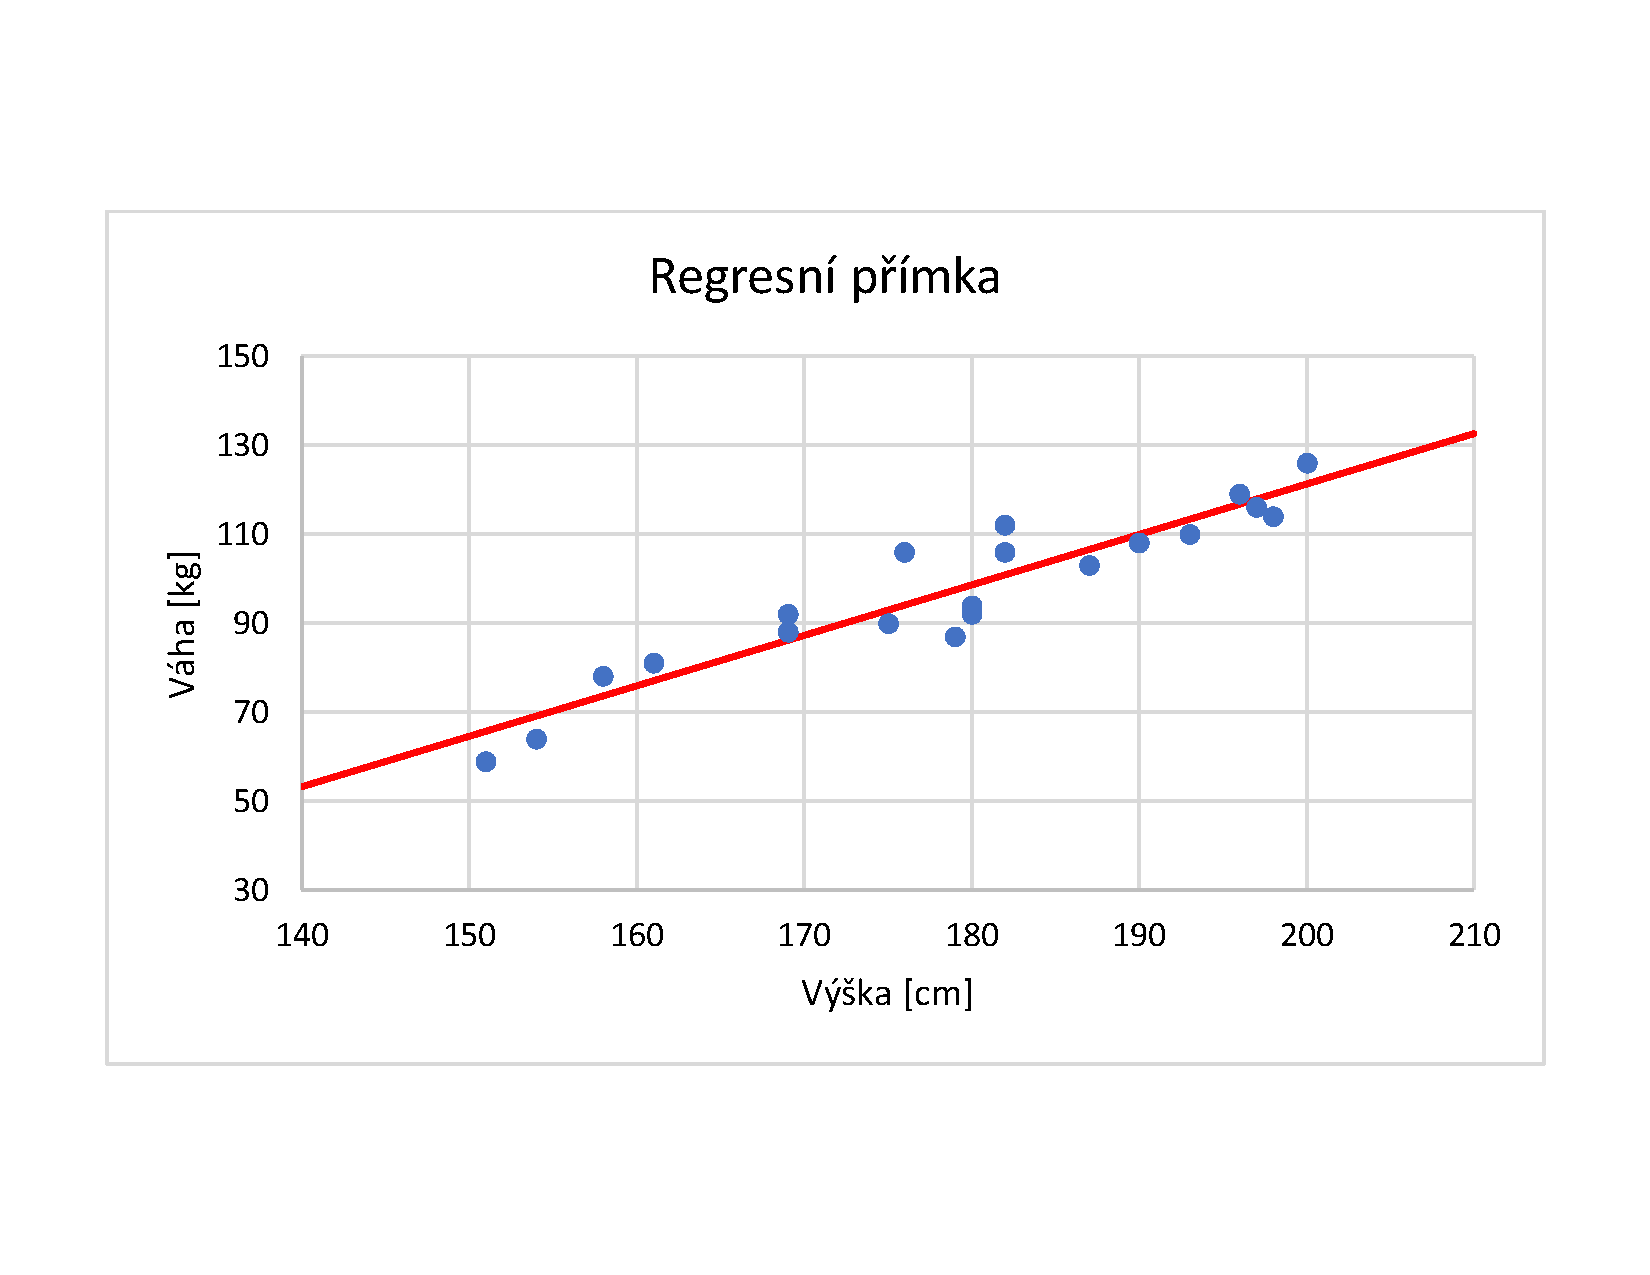
\includegraphics[width=.9\linewidth]{2-c-2-crop.pdf}
\end{figure}
\bigskip

\begin{figure}[H]
    \centering
    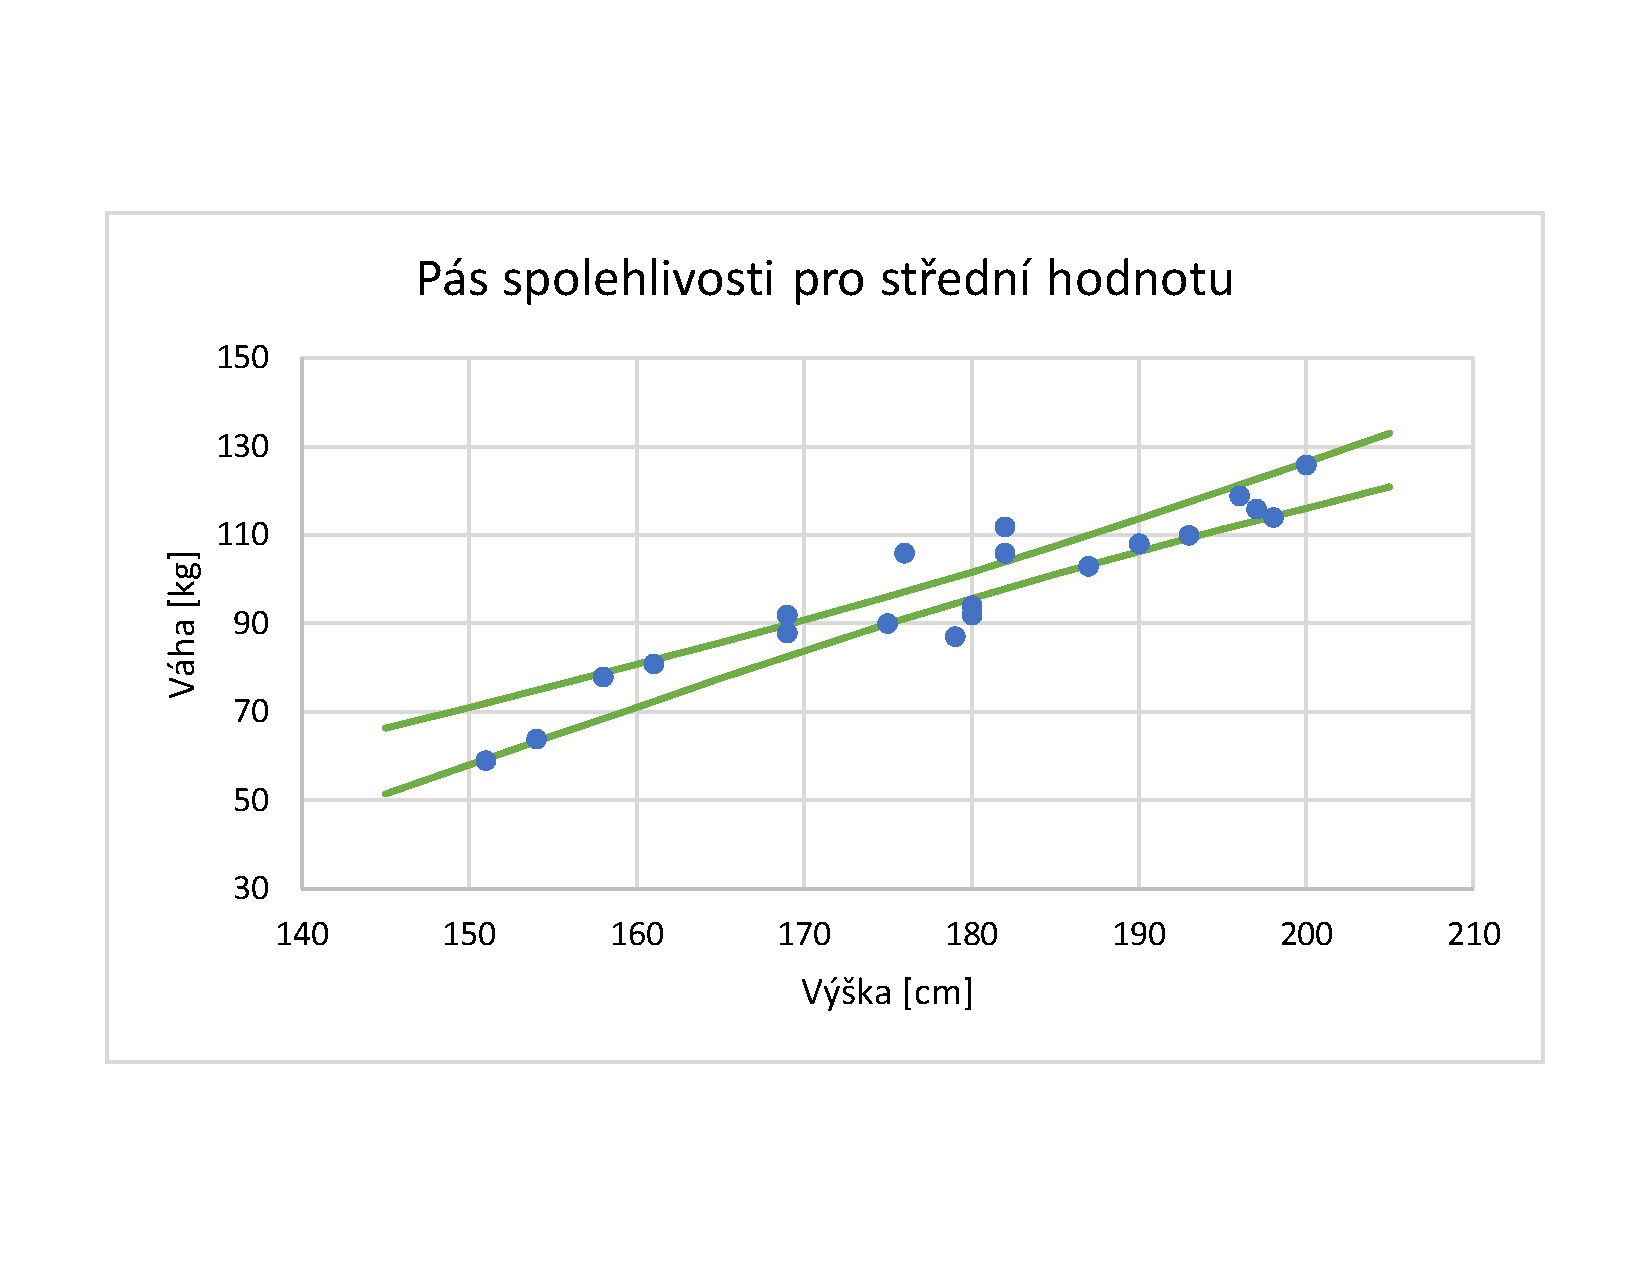
\includegraphics[width=.9\linewidth]{2-c-3-crop.pdf}
\end{figure}
\bigskip

\begin{figure}[H]
    \centering
    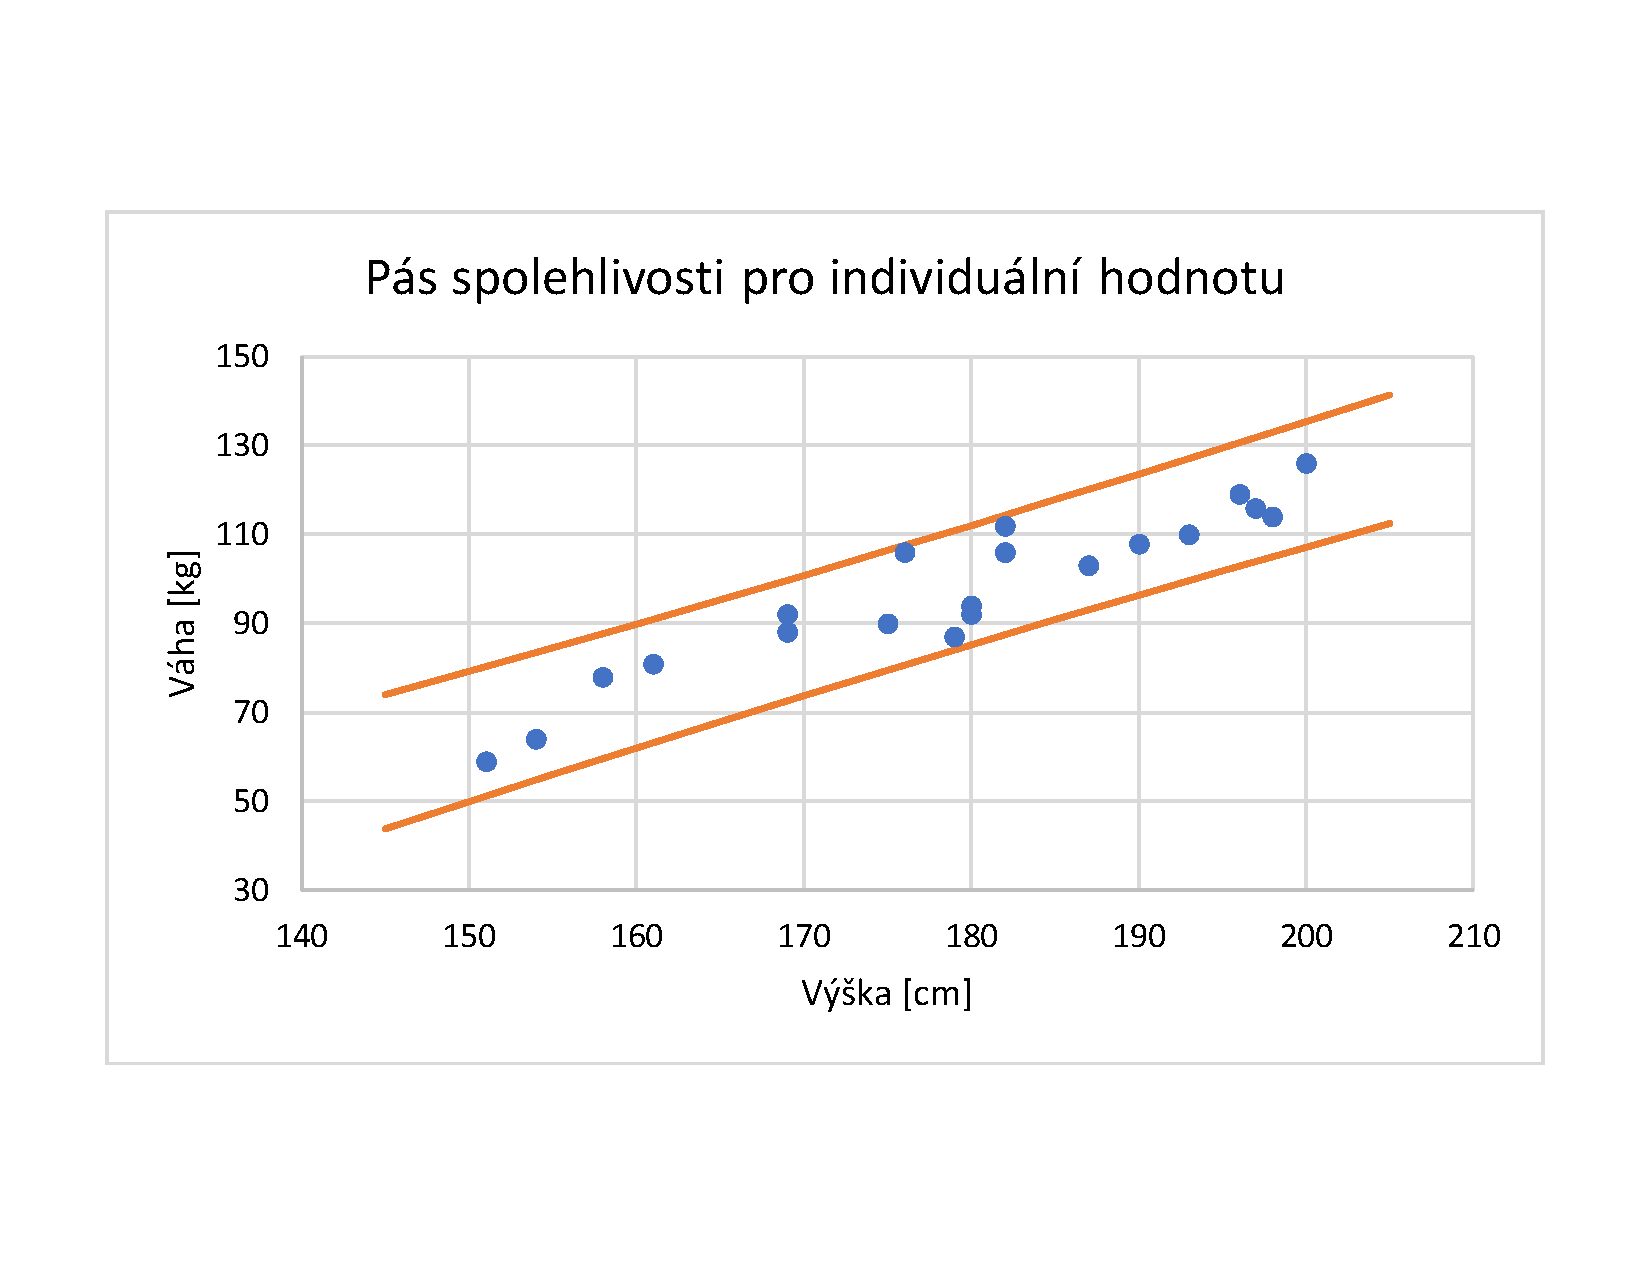
\includegraphics[width=.9\linewidth]{2-c-4-crop.pdf}
\end{figure}
